
\section{Unordered vs. Syntactic Composition}
\label{sec:model}

\begin{figure*}[t]
  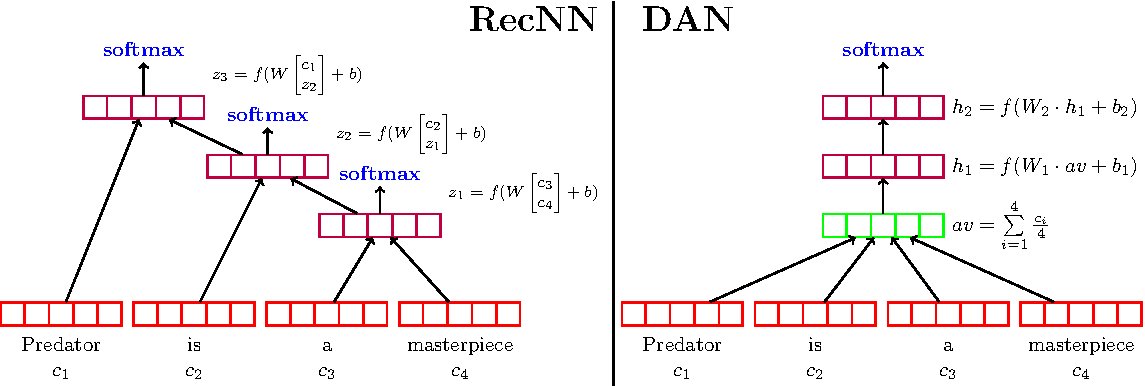
\includegraphics[scale=0.8]{2015_acl_dan/figures/dan_recnn_actualfinal.pdf}
  \caption{On the left, a \recnn\ is given an input sentence for sentiment
          classification. Softmax layers are placed above every internal node to
          avoid vanishing gradient issues. On the right is a two-layer
          \dan\ taking the same input. While the \recnn\ has to compute a
          nonlinear representation (purple vectors) for every node in the parse tree of its
          input, this \dan\ only computes two nonlinear layers for every
          possible input. }
  \label{fig:dan}
\end{figure*}


























Our goal is to marry the speed of unordered functions with the accuracy of
syntactic functions. In this section, we first describe a
class of unordered composition functions dubbed ``neural bag-of-words models''
(\nbow). We then explore more complex syntactic functions designed to avoid many
of the pitfalls associated with \nbow\ models. Finally, we present the deep
averaging network (\dan), which stacks nonlinear layers over the
traditional \nbow\ model and achieves performance on par with or better than
that of syntactic functions.

\subsection{Neural Bag-of-Words Models}\label{sec:nbow}

For simplicity, consider text classification: map an input sequence
of tokens $X$ to one of $k$ labels.  We first apply a composition
function $g$ to the sequence of word embeddings $\boldsymbol{v}_w$ for $w\in X$.
The output of this composition function is a vector $\boldsymbol{z}$ that serves
as input to a logistic regression function.





In our instantiation of \nbow, $g$ averages word embeddings\footnote{Preliminary
  experiments indicate that averaging outperforms the vector sum used in
 \nbow\ from~\newcite{kalchbrenner2014convolutional}.}


\begin{equation}\label{eq:ave}
\boldsymbol{z} = g(w \in X) = \frac 1 {\norm{X}} {\sum_{w \in X} \boldsymbol{v}_w}.
\end{equation}
Feeding $\boldsymbol{z}$ to a softmax layer induces estimated probabilities for each output label
\begin{equation}\label{eq:2}
	\hat y = \mbox{softmax}(\text{\textbf{W}}_s\cdot \boldsymbol{z} + \boldsymbol{b}),
\end{equation}
where the softmax function is
\begin{equation}\label{eq:softmax}
	\mbox{softmax}(\boldsymbol{q}) =  \frac{\exp{\boldsymbol{q}}}{\sum_{j=1}^k \exp{\boldsymbol{q}_j}}
\end{equation}
$\text{\textbf{W}}_s$ is a $k\times d$ matrix for a dataset with $k$ output
labels, and $\boldsymbol{b}$ is a bias term.




We train the \nbow\ model to minimize cross-entropy error, which for a single
training instance with ground-truth label $y$ is
\begin{equation}\label{eq:crossent}
	\ell (\hat y) = \sum\limits_{p=1}^k y_p\log(\hat y_p).
\end{equation}

Before we describe our deep extension of the \nbow\ model, we take a quick
detour to discuss syntactic composition functions.  Connections to other
representation frameworks are discussed further in Section~\ref{sec:experiments}.

\subsection{Considering Syntax for Composition}\label{sec:syntax}








Given a sentence like ``You'll be more entertained getting
hit by a bus'', an unordered model like \nbow\ might be deceived by the word ``entertained''
to return a positive prediction.  In contrast, syntactic composition functions
rely on the order and structure of the input to learn how one word or phrase
affects another, sacrificing computational efficiency in the process. In subsequent sections, we argue that this complexity is not matched by a corresponding gain in
performance.





Recursive neural networks (\recnn s) are syntactic functions that rely on natural language's inherent structure to achieve state-of-the-art accuracies on sentiment analysis tasks~\cite{taiacl15}. As in \nbow{}, each word type has an associated embedding. However, the composition function $g$ now depends on a \emph{parse tree} of the input sequence. The representation for any internal node in a binary parse tree is computed as a nonlinear function of the representations of its children (Figure~\ref{fig:dan}, left). A more powerful \recnn\ variant is the recursive neural tensor network (\rntn), which modifies $g$ to include a costly tensor product~\cite{socher2013recursive}.
















While \recnn s can model complex linguistic phenomena like
negation~\cite{Hermann:2013:CVSC}, they require much more training time than
\nbow\ models.  The nonlinearities and matrix/tensor products at each node of
the parse tree are expensive, especially as model dimensionality
increases. \recnn s also require an error signal at \emph{every} node.  One root
softmax is not strong enough for the model to learn compositional relations and leads to worse accuracies than standard bag-of-words models~\cite{jiweirnn}.
Finally, \recnn s require relatively consistent syntax between
training and test data due to their reliance on parse trees and thus cannot
effectively incorporate out-of-domain data, as we show in our question-answering
experiments. \newcite{kim:2014:EMNLP2014} shows that some of these issues can be avoided by using a convolutional network instead of a \recnn, but the computational complexity increases even further (see Section~\ref{sec:experiments} for runtime comparisons).

What contributes most to the power of syntactic functions: the compositionality
or the nonlinearities? \newcite{socher2013recursive} report that
removing the nonlinearities from their \recnn\ models drops performance on the
Stanford Sentiment Treebank by over 5\% absolute accuracy. Most unordered functions are linear
mappings between bag-of-words features and output labels, so might they suffer
from the same issue? To isolate the effects of syntactic composition from the
nonlinear transformations that are crucial to \recnn\ performance, we
investigate how well a deep version of the \nbow\ model performs on tasks that
have recently been dominated by syntactically-aware models.
